\section{Tutela Overview}
\label{sec:tutela}

Tutela\footnote{At the time of publication, Tutela is hosted at \url{https://www.tutela.xyz}.}, latin for protection, is a web application that has three functions, it inform users which of their Ethereum addresses are affiliated, how they are linked and audits the anonymity sets of Tornado Cash Pools. More on each of these below.

\subsection {Ethereum Address Clustering}

Users can search an ethereum address (e.g. 0x...) or ENS (e.g. tutela.eth), and receive a summary of its anonymity. 

\begin{figure}[h!]
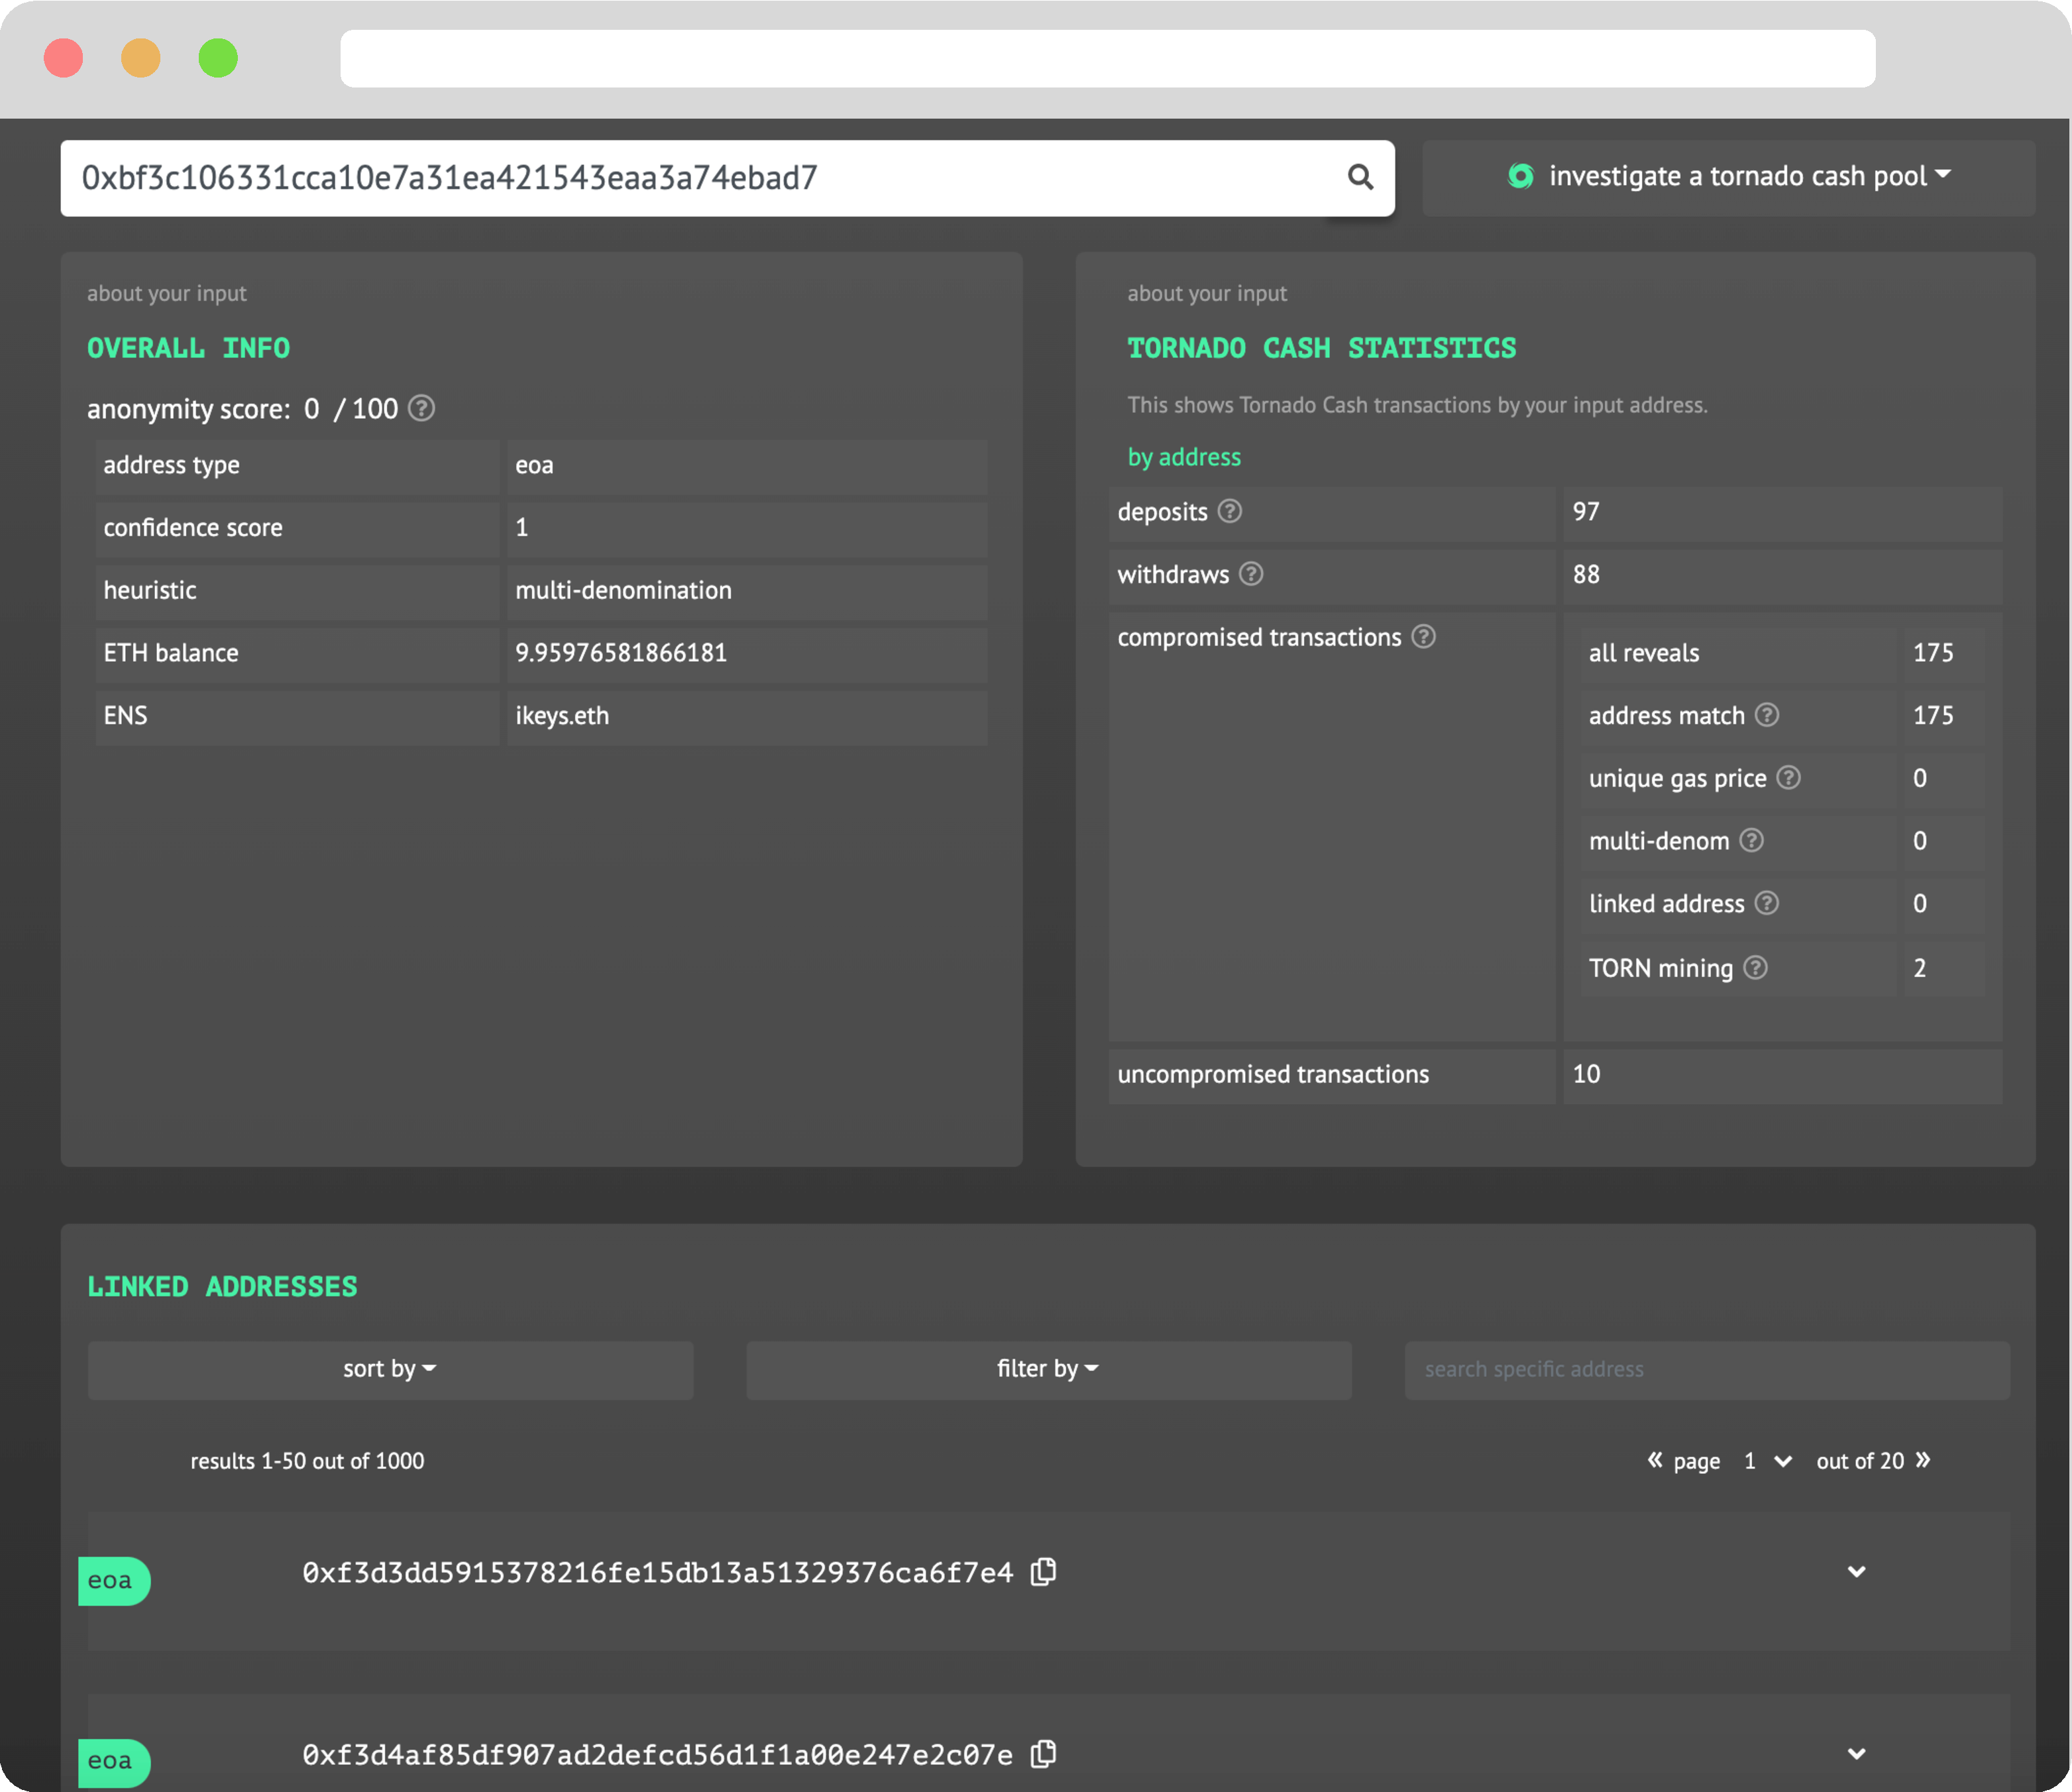
\includegraphics[width=\linewidth]{figures/demo.pdf}
\caption{Tutela address page when searching an Ethereum address. This address is also a TC user.}
\end{figure}

We summarize the main functionalities shown in Figure~\ref{fig:demo}. The response page is separated into three sections. The top left section summarizes the anonymity of the searched address. It contains an ``anonymity score'' out of 100, where a lower number represents less anonymity. In this example, the searched address has an anonymity score of 0, representing a large amount of leaked identity information. Other information, such as balance in ETH or ENS names, are shown when relevant.

The top right section is only populated if the searched address is a Tornado Cash user. In this example, the searched address has deposited 97 times to a Tornado Cash pool and withdrawn 88 times. Interestingly, we find that through heuristics, we are able to tie 87 of those withdraw transactions to deposit transactions, thereby meaningfully reducing the useful size of the Tornado Cash pool. See Section~\ref{sec:tornado} for more details.

The bottom section labeled ``Linked Addresses'' shows a list of addresses clustered with the searched one. Each item in this list is denoted as either an externally owned address (EOA), a deposit address, or an exchange address. Each item also contains a confidence score denoting the strength of association with the searched address, and the heuristic that bound it to the searched address.
This example shows a thousand clustered addresses representing an entity with a large wallet portfolio (e.g., bot) -- hence why the anonymity score is zero.

\subsection{Ethereum Address Reveals}

\begin{figure}[h!]
\includegraphics[width=\linewidth]{figures/demo3.pdf}
\caption{Tutela transaction page when searching an Ethereum address. This address is also a TC user.}
\label{fig:demo3}
\end{figure}

To see a history of when an Ethereum user potentially committed reveals, users can select the transactions tab on the landing page and input an Ethereum address or ENS. The right hand side of Figure~\ref{fig:demo3} shows a graph of when these revealing transactions occurred where the x-axis denotes the weeks prior to the current date. Each bar in the graph corresponds to an individual week and upon clicking on each bar, Tutela will show the details of the potentially revealing transactions underneath. On the left hand side, users can see statistics on their potential reveals as well as a comparison to the average Tornado Cash user. 


\subsection{Tornado Cash Anonymity Set Auditor}

The Tornado Cash Anonymity Set Auditor, computes the five heuristics described in Section~\ref{sec:tornado} for each Tornado Cash pool to determine how many potentially compromised deposits are in each pool.

\begin{figure}[h!]
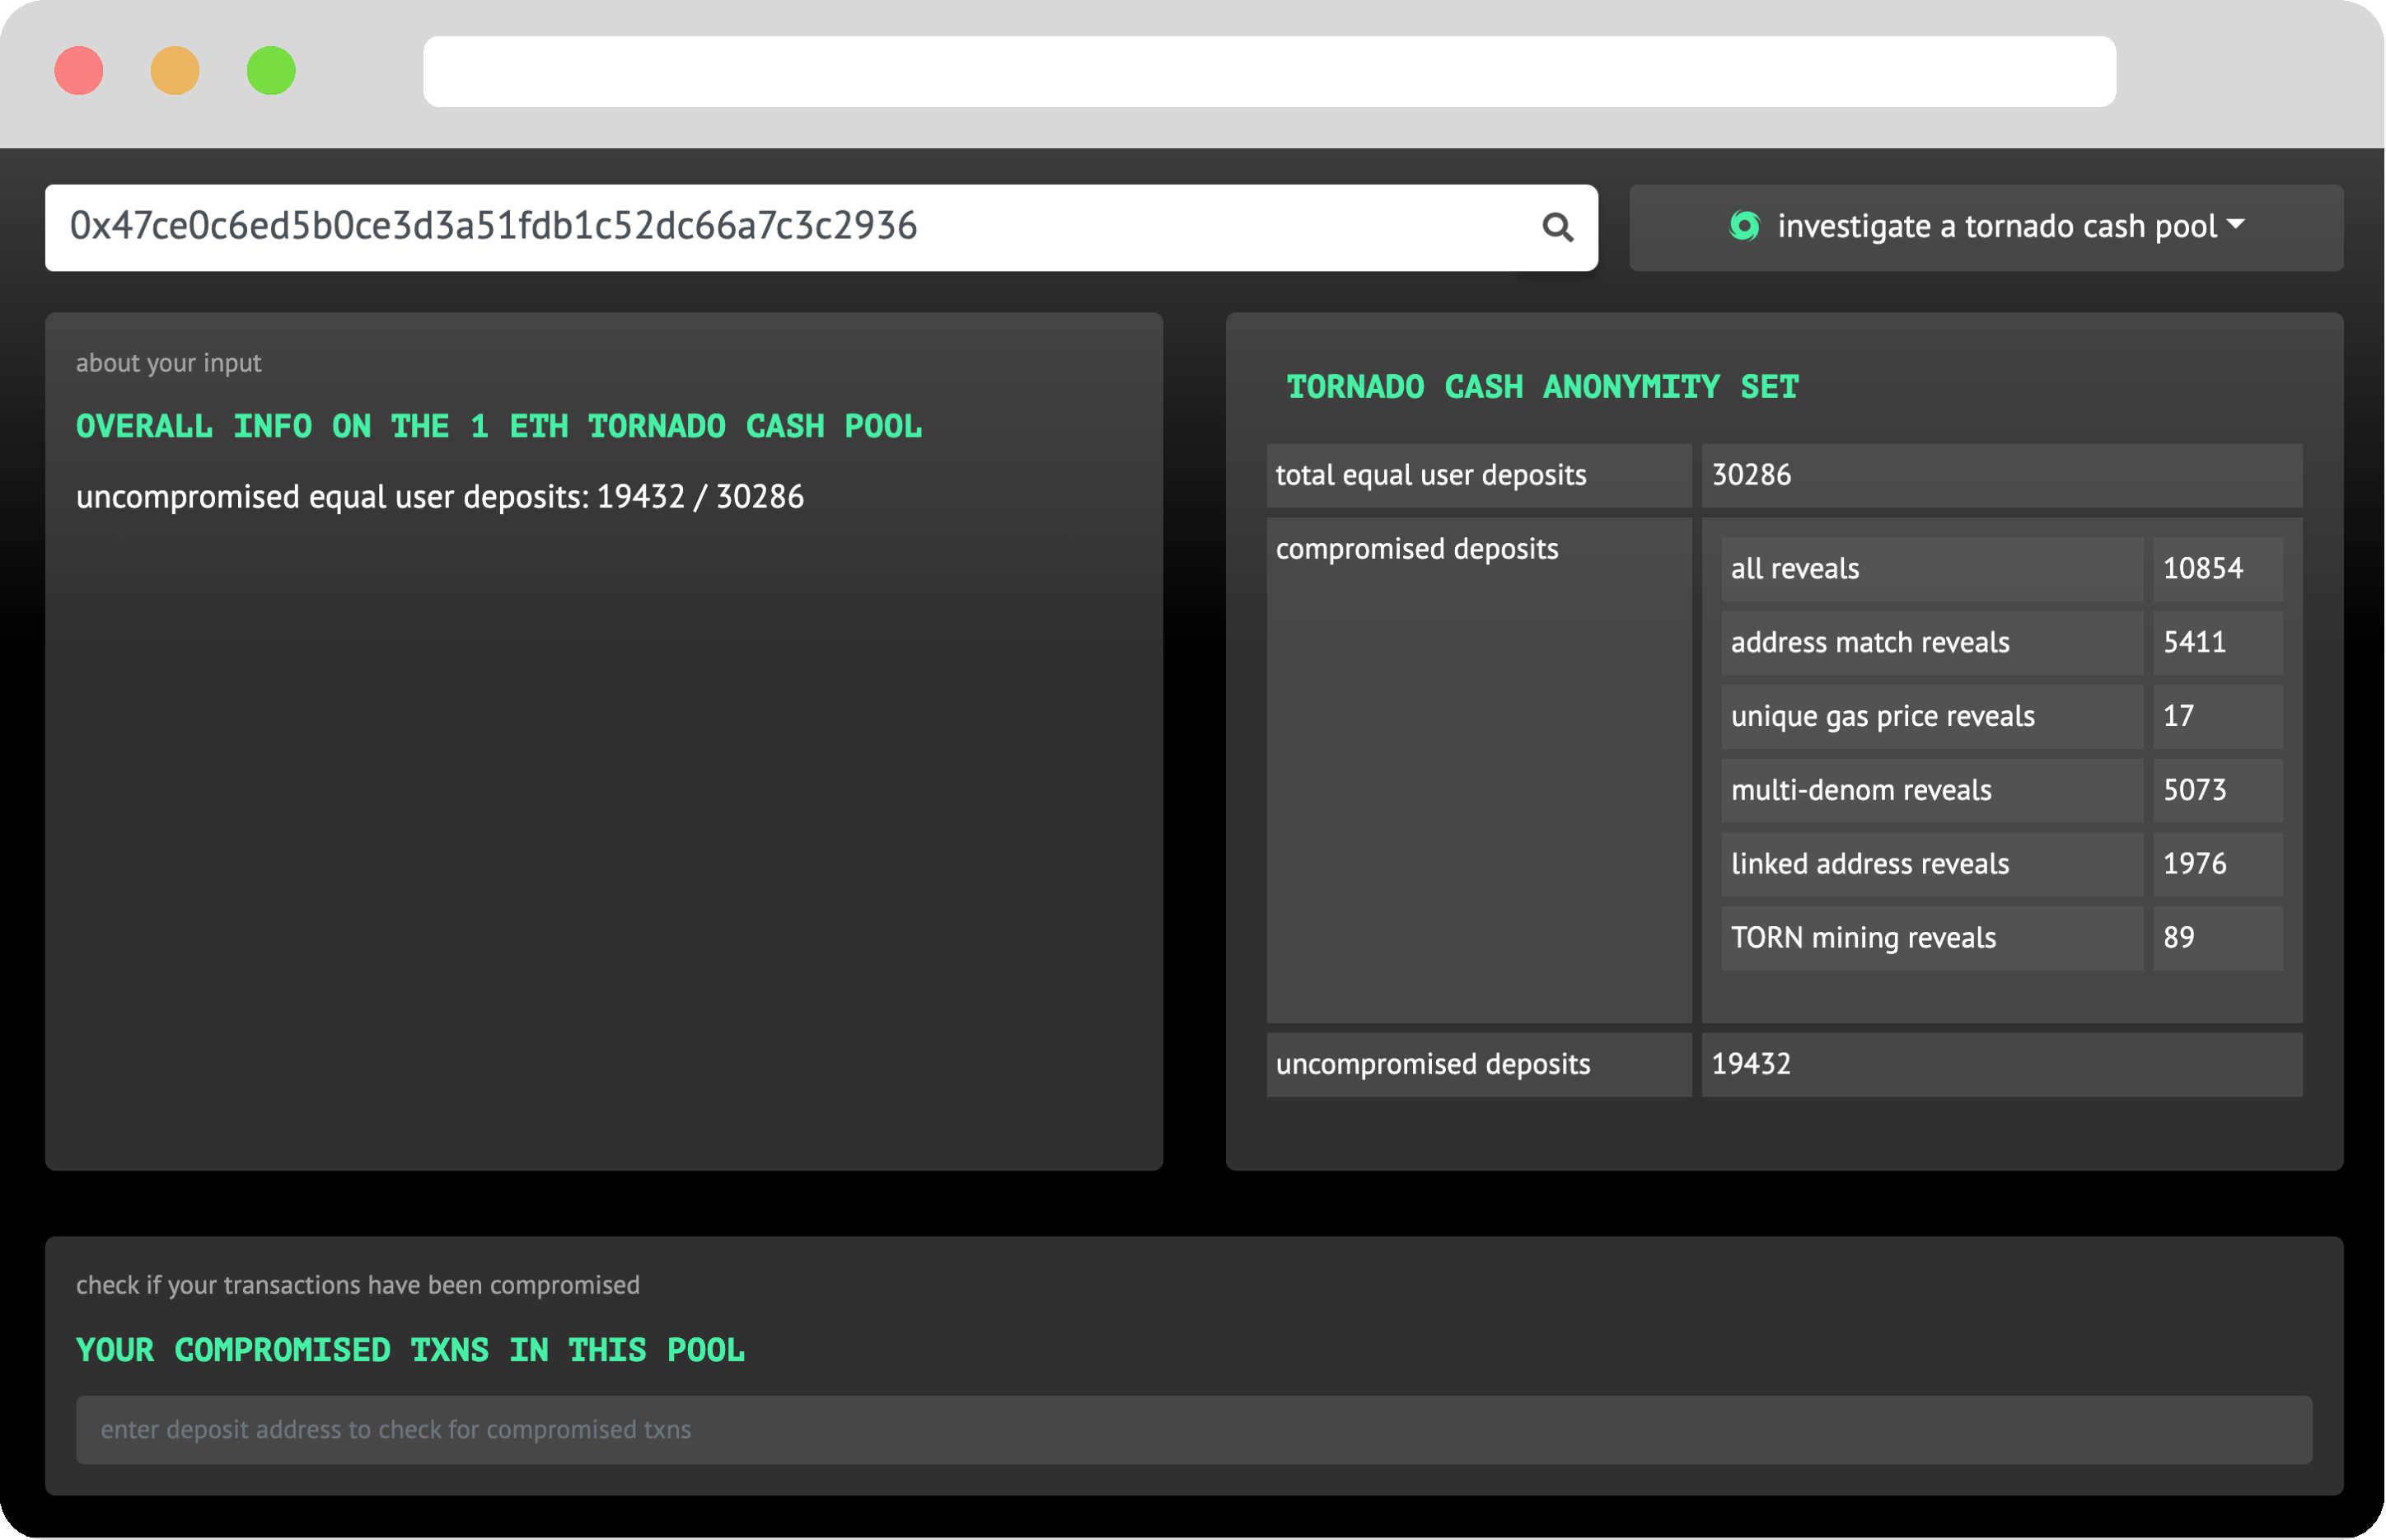
\includegraphics[width=\linewidth]{figures/demo2.pdf}
\caption{Tutela interface when searching a Tornado Cash pool.}
\label{fig:demo2}
\end{figure}

If a user selects a Tornado Cash Pool from the dropdown list on the landing page, the top right of the results page will show the headline number of equal user deposits in a Tornado Cash pool, otherwise known as its anonymity set. Below that, we compute the ``true'' anonymity set size for the pool, subtracting out all equal user deposits that may have been compromised through our heuristics. This gives the number of “uncompromised deposits”. At the time of publication, the Tornado Cash website reports only the full anonymity set size, not taking into account potential compromises. 

At the bottom of Figure~\ref{fig:demo2}, users can supply an address to check, \textit{in a private way}, if it has made any compromising transactions, inspired by the popular website ``Have I been pwned?''\footnote{See \url{https://haveibeenpwned.com}.}.

A concrete use case of Tutela is to adjust anonymity set to protect the privacy of Tornado Cash users more faithfully. As described in Section~\ref{sec:preliminaries}, if a pool has many compromised deposits, it provides less privacy than a user believes.